\documentclass{article}
\usepackage{enumerate}
\usepackage{amsmath}
\usepackage{amssymb}
\usepackage{graphicx}
\usepackage{subfigure}
\usepackage{geometry}
\usepackage{caption}
\usepackage{indentfirst}
\usepackage{array}
%\renewcommand\arraystretch{2}
\usepackage{tikz}
\usepackage{multicol}
\usepackage{algorithm}
\usepackage{algorithmicx}
\usepackage{algpseudocode}
\renewcommand{\algorithmicrequire}{\textbf{Input:}}
\renewcommand{\algorithmicensure}{\textbf{Output:}}
\usepackage{minted}
\usemintedstyle{autumn}
\geometry{left=3.0cm,right=3.0cm,top=3.0cm,bottom=4.0cm}
\renewcommand{\thesection}{Ex. \arabic{section}}
\title{VE281 Writing Assignment Five}
\author{Liu Yihao 515370910207}
\date{}

\begin{document}
\maketitle

\section{}
\begin{enumerate}[(a)]
\item\
\begin{center}
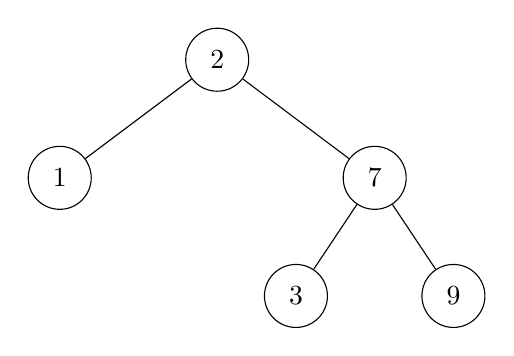
\begin{tikzpicture}
\tikzstyle{every node}=[draw,shape=circle,minimum size=0.8cm];
\node {2}[sibling distance=4cm]
child { node {1}[sibling distance=2cm]
}
child {
	node {7}[sibling distance=2cm]
	child {
		node {3}
	}
	child {
		node {9}
	}
};
\end{tikzpicture}
\end{center}
\item\
\begin{center}
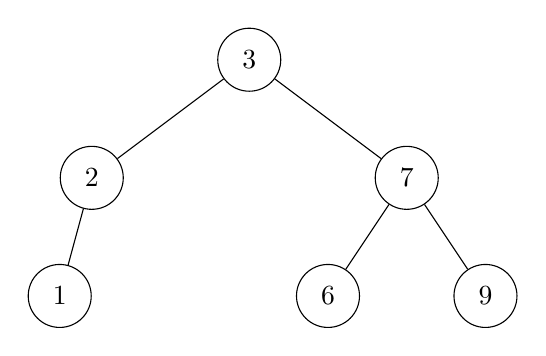
\begin{tikzpicture}
\tikzstyle{every node}=[draw,shape=circle,minimum size=0.8cm];
\node {3}[sibling distance=4cm]
child {
	node {2}[sibling distance=2cm]
	child[left] {
		node {1}
	}
}
child {
	node {7}[sibling distance=2cm]
	child {
		node {6}
	}
	child {
		node {9}
	}
};
\end{tikzpicture}
\end{center}
\item\
\begin{center}
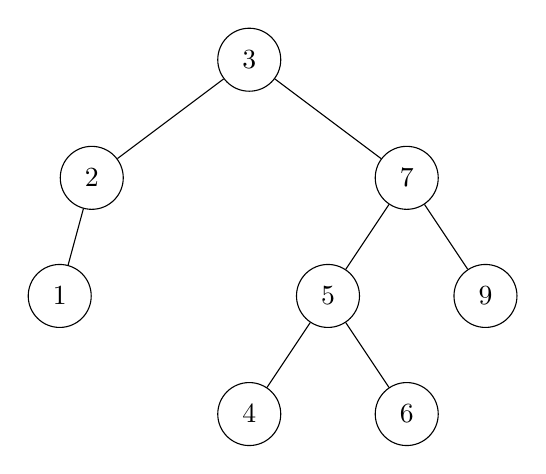
\begin{tikzpicture}
\tikzstyle{every node}=[draw,shape=circle,minimum size=0.8cm];
\node {3}[sibling distance=4cm]
child {
	node {2}[sibling distance=2cm]
	child[left] {
		node {1}
	}
}
child {
	node {7}[sibling distance=2cm]
	child {
		node {5}
		child {
			node {4}
		}
		child {
			node {6}
		}
	}
	child {
		node {9}
	}
};
\end{tikzpicture}
\end{center}
\item\
\begin{center}
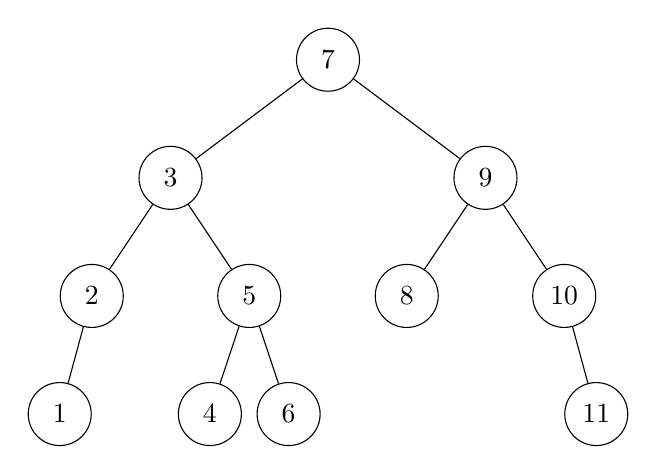
\begin{tikzpicture}
\tikzstyle{every node}=[draw,shape=circle,minimum size=0.8cm];
\node {7}[sibling distance=4cm]
child {
	node {3}[sibling distance=2cm]
	child {
		node {2}[sibling distance=1cm]
		child[left] {
			node {1}
		}
	}
	child {
		node {5}[sibling distance=1cm]
		child {
			node {4}
		}
		child {
			node {6}
		}
	}
}
child {
	node {9}[sibling distance=2cm]
	child {
		node {8}
	}
	child {
		node {10}[sibling distance=1cm]
		child[right] {
			node {11}
		}
	}
};
\end{tikzpicture}
\end{center}
\item\
\begin{center}
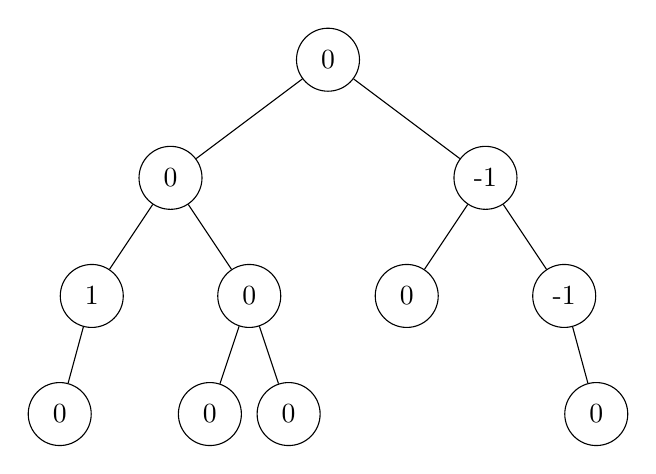
\begin{tikzpicture}
\tikzstyle{every node}=[draw,shape=circle,minimum size=0.8cm];
\node {0}[sibling distance=4cm]
child {
	node {0}[sibling distance=2cm]
	child {
		node {1}[sibling distance=1cm]
		child[left] {
			node {0}
		}
	}
	child {
		node {0}[sibling distance=1cm]
		child {
			node {0}
		}
		child {
			node {0}
		}
	}
}
child {
	node {-1}[sibling distance=2cm]
	child {
		node {0}
	}
	child {
		node {-1}[sibling distance=1cm]
		child[right] {
			node {0}
		}
	}
};
\end{tikzpicture}
\end{center}
\end{enumerate}

\section{}
The node filled in white means red node, The node filled in black means black node.

\begin{enumerate}[(a)]
\item\
\begin{center}
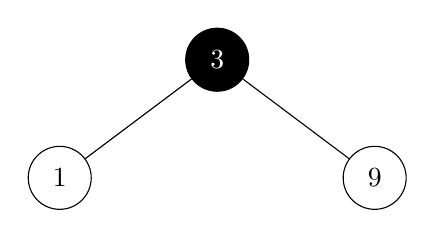
\begin{tikzpicture}
\tikzstyle{every node}=[draw,shape=circle,minimum size=0.8cm];
\node[fill=black] {\textcolor{white}{3}}[sibling distance=4cm]
child {
	node {1}[sibling distance=2cm]
}
child {
	node {9}[sibling distance=2cm]
};
\end{tikzpicture}
\end{center}
\item\
\begin{center}
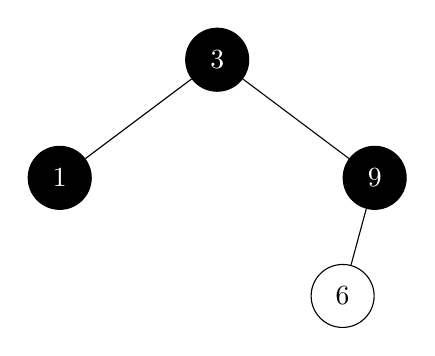
\begin{tikzpicture}
\tikzstyle{every node}=[draw,shape=circle,minimum size=0.8cm];
\node[fill=black] {\textcolor{white}{3}}[sibling distance=4cm]
child {
	node[fill=black] {\textcolor{white}{1}}[sibling distance=2cm]
}
child {
	node[fill=black] {\textcolor{white}{9}}[sibling distance=2cm]
	child[left] {
		node {6}
	}
};
\end{tikzpicture}
\end{center}
\item\
\begin{center}
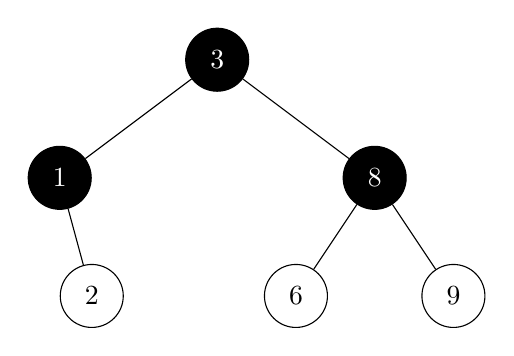
\begin{tikzpicture}
\tikzstyle{every node}=[draw,shape=circle,minimum size=0.8cm];
\node[fill=black] {\textcolor{white}{3}}[sibling distance=4cm]
child {
	node[fill=black] {\textcolor{white}{1}}[sibling distance=2cm]
	child[right] {
		node {2}
	}
}
child {
	node[fill=black] {\textcolor{white}{8}}[sibling distance=2cm]
	child {
		node {6}
	}
	child {
		node {9}
	}
};
\end{tikzpicture}
\end{center}
\item\
\begin{center}
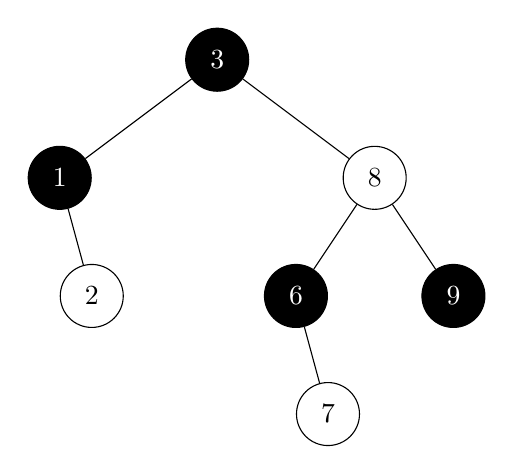
\begin{tikzpicture}
\tikzstyle{every node}=[draw,shape=circle,minimum size=0.8cm];
\node[fill=black] {\textcolor{white}{3}}[sibling distance=4cm]
child {
	node[fill=black] {\textcolor{white}{1}}[sibling distance=2cm]
	child[right] {
		node {2}
	}
}
child {
	node {8}[sibling distance=2cm]
	child {
		node[fill=black] {\textcolor{white}{6}}
		child[right] {
			node {7}
		}
	}
	child {
		node[fill=black] {\textcolor{white}{9}}
	}
};
\end{tikzpicture}
\end{center}
\item\
\begin{center}
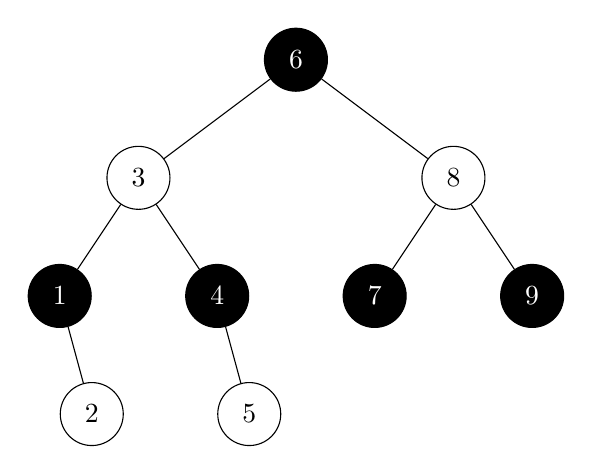
\begin{tikzpicture}
\tikzstyle{every node}=[draw,shape=circle,minimum size=0.8cm];
\node[fill=black] {\textcolor{white}{6}}[sibling distance=4cm]
child {
	node {3}[sibling distance=2cm]
	child {
		node[fill=black] {\textcolor{white}{1}}[sibling distance=1cm]
		child[right] {
			node {2}
		}
	}
	child {
		node[fill=black] {\textcolor{white}{4}}[sibling distance=1cm]
		child[right] {
			node {5}
		}
	}
}
child {
	node {8}[sibling distance=2cm]
	child {
		node[fill=black] {\textcolor{white}{7}}
	}
	child {
		node[fill=black] {\textcolor{white}{9}}
	}
};
\end{tikzpicture}
\end{center}
\end{enumerate}

\section{}
In a tree of $n$ nodes, there are at most $n-1$ left nodes. For each left node, if it is a leaf, we can do a right rotation on its parent so that there is one less left node and one more right node, and left nodes which are not leaves may become leaves. Repeat this procedure and there will be $n-1$ right leaves. Note that this procedure is invertible, so every two tree both can be transformed into a right-skewed tree in $n-1$ rotations, so $2n-2$ rotations needed to transform one tree into another. The complexity is $O(n)$.

\section{}
\begin{enumerate}
\item\
\begin{center}
\begin{tikzpicture}
\tikzstyle{every node}=[draw,shape=circle,minimum size=0.8cm];
\node [label={$h=X+1$}]{P}[sibling distance=4cm]
child {
	node [label={$h=X$}]{A}[sibling distance=2cm]
}
child {
	node [label={$h=X-1$}]{B}[sibling distance=2cm]
};
\end{tikzpicture}
\end{center}

If the height of $A$ doesn't change after the insertion, a balance condition violation won't occur. So the height of $A$ becomes $X+1$ after the insertion, and the balance factor of $P$ becomes 2.

\item\
\begin{center}
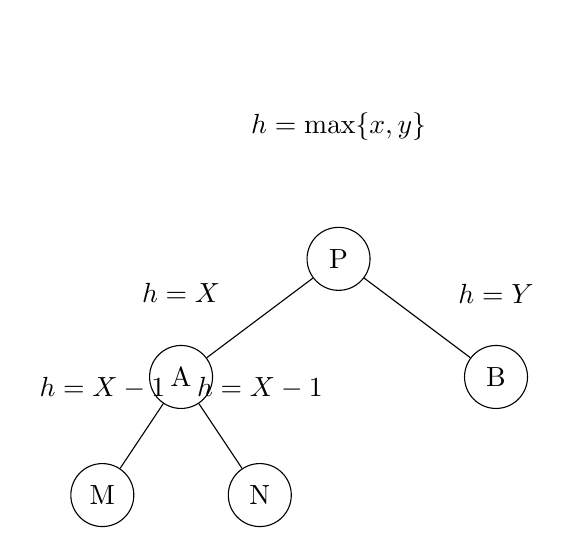
\begin{tikzpicture}
\tikzstyle{every node}=[draw,shape=circle,minimum size=0.8cm];
\node [label={$h=\max\{x,y\}$}]{P}[sibling distance=4cm]
child {
	node [label={$h=X$}]{A}[sibling distance=2cm]
	child {
		node [label={$h=X-1$}]{M}
	}
	child {
		node [label={$h=X-1$}]{N}
	}
}
child {
	node [label={$h=Y$}]{B}[sibling distance=2cm]
};
\end{tikzpicture}
\end{center}

If the height of $M$ or $N$ doesn't change after the insertion, a balance condition violation won't occur. So the height of $M$ or $N$ becomes $X$ after the insertion, and the balance factor of $A$ becomes $\pm1$.

\end{enumerate}

\end{document}
